\chapter{可行性分析结果}

本部分将进行对本网盘主体结构的可行性分析,具体内容分客户端、服务器和web服务器以及web应用程序三者的交互网页三个部分。

\section{客户端}

本项目的Java客户端是一个服务程序,与服务器基于tcp协议的socket通信建立连接。客户端通过配置文件来进行配置。配置文件会选择要进行共享的文件列表,并提供服务器的IP接口。

可使用PropertiesLoaderUtils工具类来进行配置文件的读取和修改,Spring 提供的 PropertiesLoaderUtils 允许直接通过基于类路径的文件地址加载属性资源,最大的好处就是:实时加载配置文件,修改后立即生效,不必重启。

Java客户端提供以下几种功能:

\textbf{1.  获取本地目录:}

服务器需要知道本地机器参与共享的文件列表,使用 java.io.File类即可操作获取。

\textbf{2.  对文件进行分块:}

当服务器发来需要分块的文件时,客户端需要对文件应用erasure code算法进行分块,分块算法已经基于backblaze开源实现。

\textbf{3.  向服务器发送文件碎片、接收服务器传来的碎片:}
当文件分块完成后,客户端便向服务器发出post请求,服务器开通数据传输端口,客户端将文件碎片发送向客户端。若有服务器发出获取碎片请求,客户端则将存在本地的碎片发向客户端。
                 
\textbf{4.  响应服务器删除本地文件:}
文件删除可以用TrackerClient类实现。

\section{服务器}

服务器程序是分布式文件系统的核心组件,其管理着整个分布式文件系统的元数据并支持客户端服务程序和动态网页与分布式文件系统的交互。

服务器程序的功能主要有接收、回复、转发服务请求与控制信息,维护云共享文件索引,转发数据,维护各个客户端的状态信息,支持动态网页和记录、处理当前等待响应的文件请求。

服务器程序的结构如下图一所示:
\begin{figure}[ht]
\centering
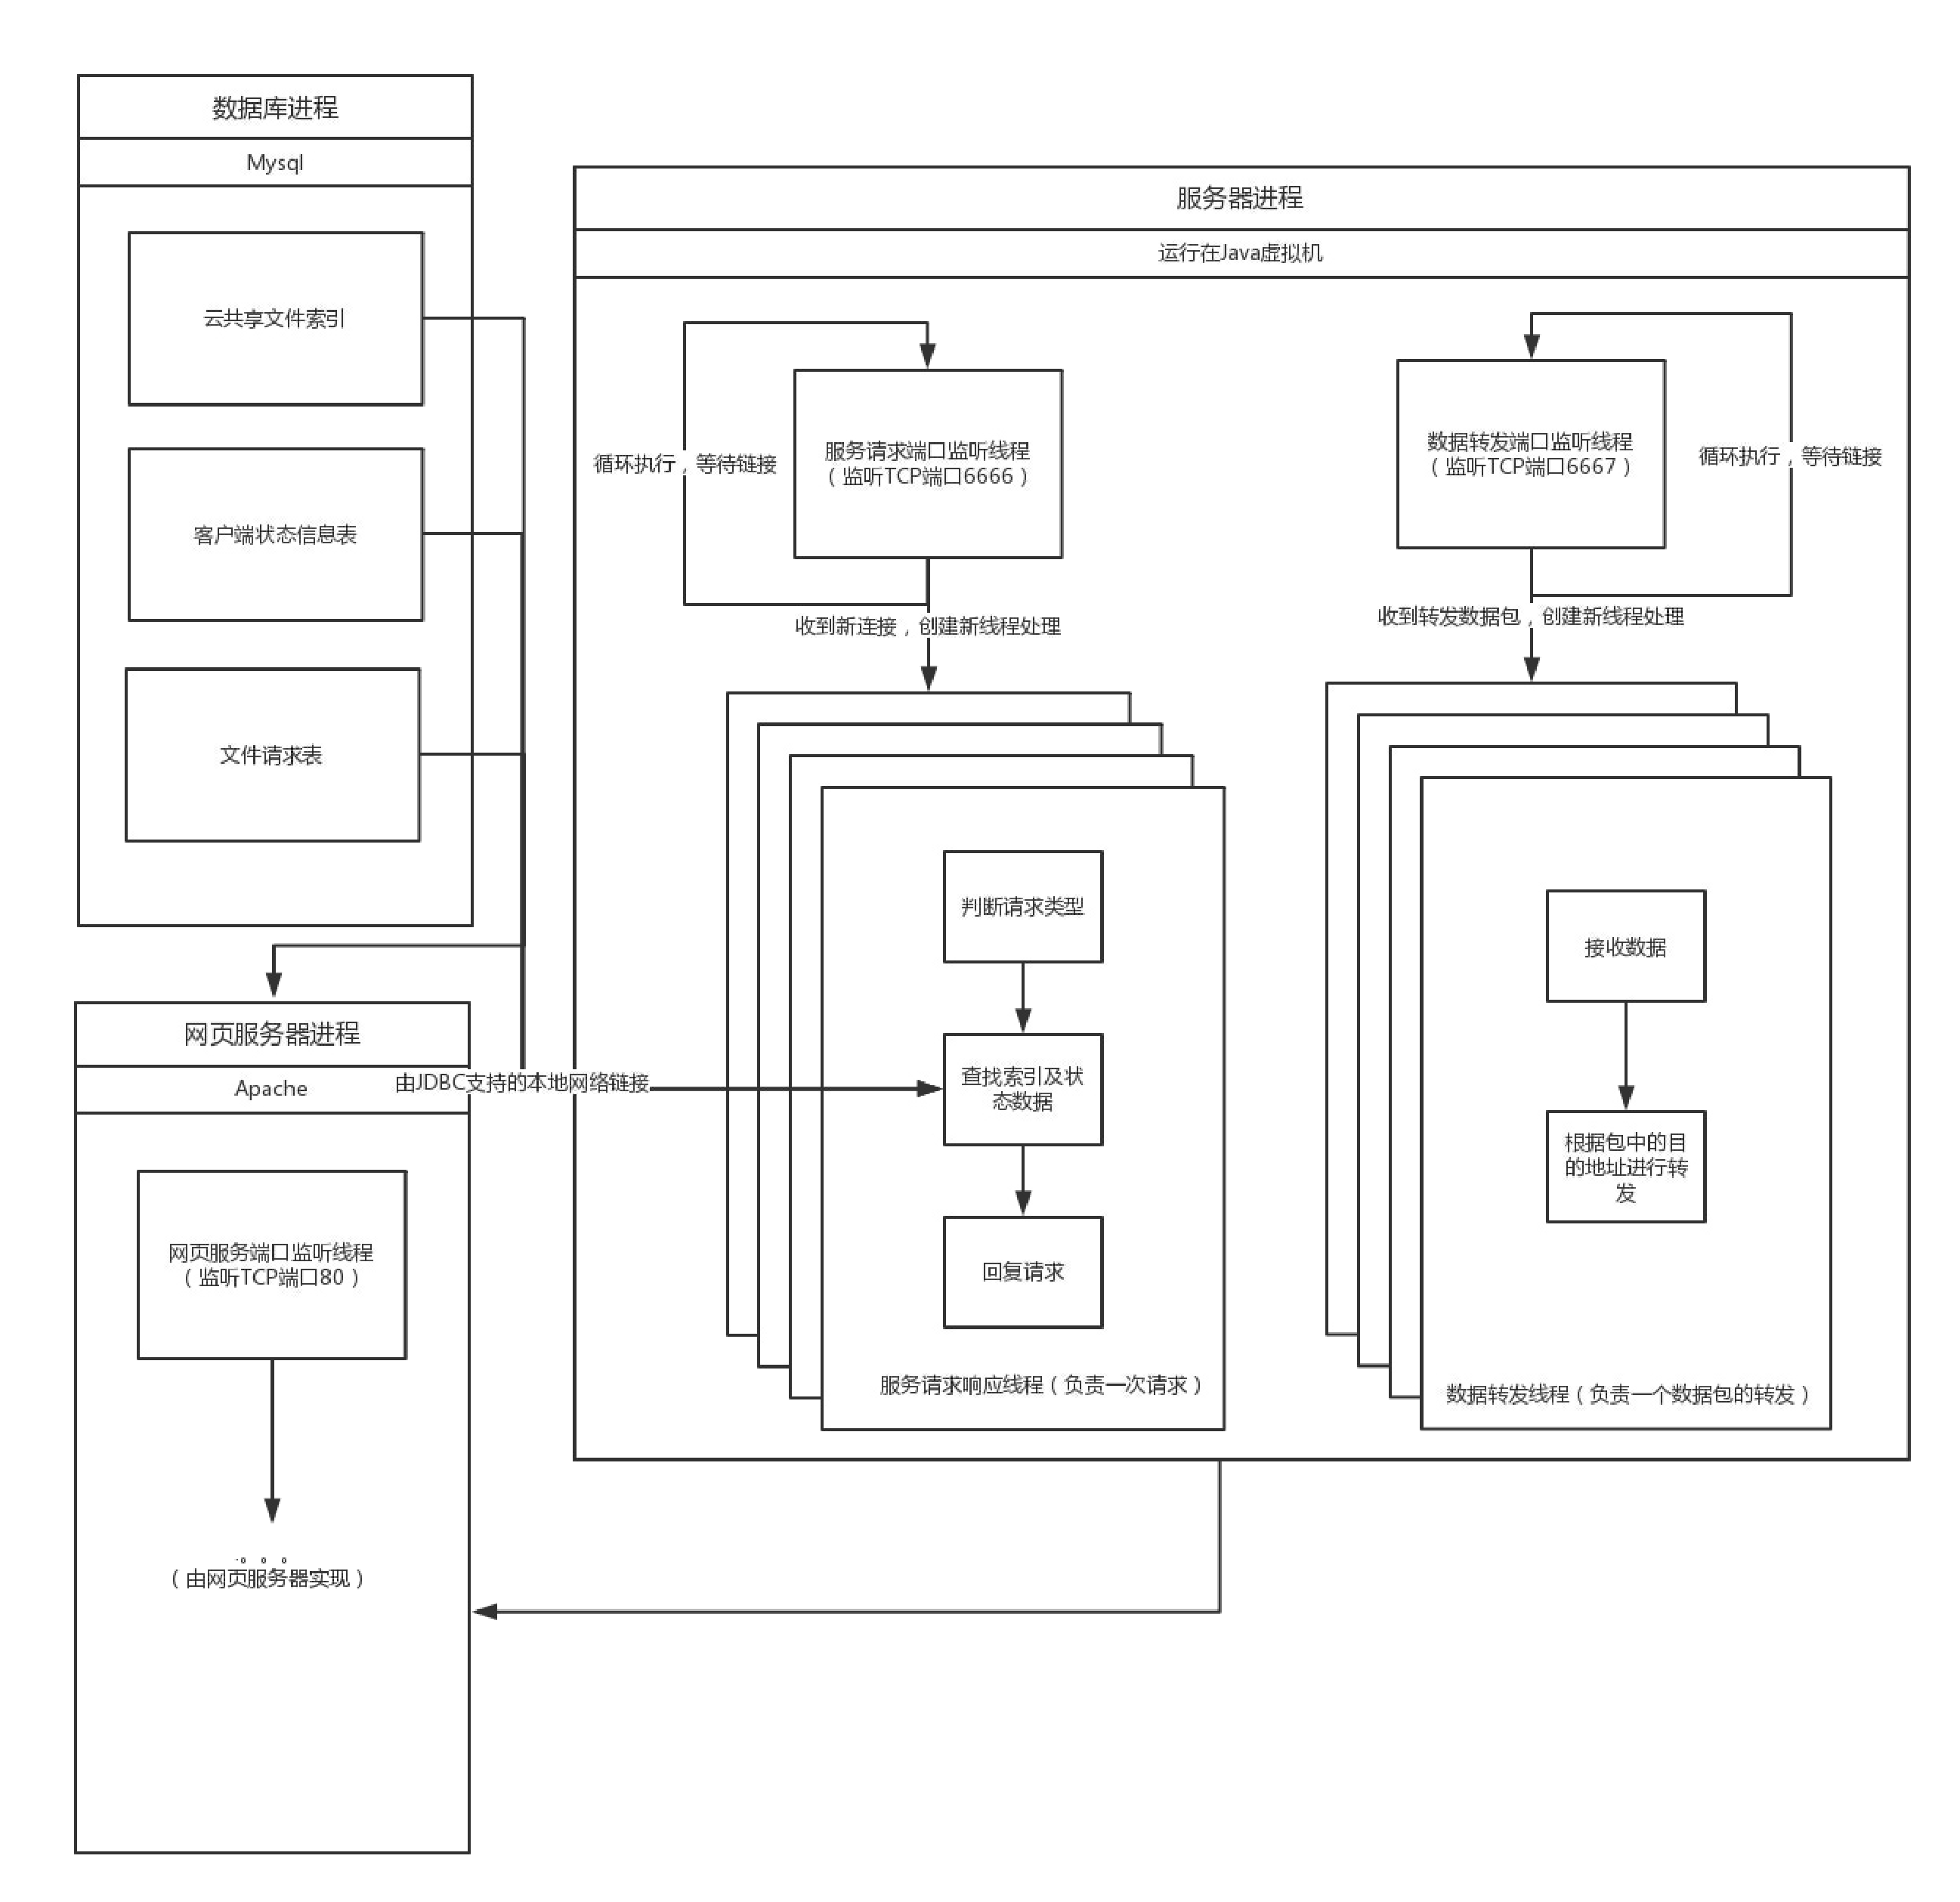
\includegraphics[width=10cm]{arch_server}
\caption{服务器结构} \label{fig:figure3}
\end{figure}

服务器程序包括两个常开的线程用于监听两个不同的TCP端口分别用来回应服务请求和转发数据,对于每个TCP链接,服务器进程将创建一个线程进行处理,这将保证服务器可以在处理一个请求时不至于失去响应。

Java提供了接口Runable供多线程编程使用,实现Runable的类只需重写run方法便可以在类中实例化一个线程(Thread类)对象,并通过start方法将这个线程提交给JVM的线程调度队列。

为了避免复杂的线程间同步与内存管理,本报告设计的分布式文件系统采用MySQL数据库保存文件索引信息和各客户端的状态信息。MySQL原本是一个开放源代码的关系数据库管理系统,原开发者为瑞典的MySQL AB公司。2008年MySQL AB公司被昇阳微系统收购,2009年,甲骨文公司收购了昇阳微系统公司,故当前MySQL为Oracle旗下产品。同其他数据库一样,MySQL可以通过标准查询语言(SQL)进行查询。

为了避免在数据库上进行漫长的线性查找,MYSQL支持为数据库添加索引。引擎为InnoDB或MyISAM的数据库支持基于B-Tree的索引,其可以将查询时间减少到O(log(n));引擎为MEMORY的数据库支持基于Hash的索引,其可以将查询时间减少到O(1))。添加索引可以通过SQL命令执行;具体数据库引擎的选择则还要考虑到数据库的大小(如MEMORY引擎的数据库大小不能超过RAM大小)和并发性的要求。

MySQL数据库支持并发操作,为了在并发操作中保持数据的一致性,MySQL提供锁机制与事务机制。MySQL的锁机制包括表级锁(锁定整张表)和行级锁(锁定特定行,并发程度更高);MySQL的事务机制保证一系列的SQL可以被原子的执行且不被其他事务干扰。不同引擎的表对并发性的支持是不同的,如InnoDB实现了行级锁而MyISAM存储引擎不支持行级锁。MySQL中InnoDB引擎支持具有事务、回滚和崩溃修复能力的事务安全型表,对并发性有最好的支持。因此,考虑到索引的速度、数据库大小的支持与对并发性的支持,本报告中设计的分布式文件系统采用基于InnoDB引擎的数据库。

Java提供了Java数据库连接(JDBC)作为规范客户端程序如何来访问数据库的应用程序接口并提供了诸如查询和更新数据库中数据的方法。只需加载MySQL的驱动,就可以在Java程序中链接MySQL数据库并通过SQL查询(或修改)数据库中的内容。

下面介绍服务器程序提供的功能。

接收、回复、转发服务请求与控制信息:服务器与客户端通过非持续的TCP链接传递HTTP报文来交换信息。

Java提供了ServerSocket类和Socket类来进行基于TCP链接的网络通信。ServerSocket类可以用于在服务器端创建一个欢迎套接字,Socket类可以在客户端或服务器端创建链接套接字。

转发数据:由于各个客户端之间未必可以直接连接(如客户端可能隐藏在NAT后),客户端有时需要通过服务器转发消息,这种情况可能有两种:

(1)当一个客户端上传了文件,其需要发送碎片到另一个客户端

(2)当网页请求文件,其需要接收各客户端的碎片

对于以上的任何一种情况,转发数据时将随数据附带目的地址,故服务器只需接收数据并将数据发送到目的地址即可。

维护云共享文件索引
云共享文件索引以MySQL数据库中的一系列table的形式保存。每个用户均在数据库中对应两个table,其一记录了这个用户的每个文件的唯一标识符和其逻辑位置;其二记录了这个用户的每个文件的各个碎片的物理位置和其唯一标识符。

维护各个客户端的状态信息
客户端状态信息以MySQL数据库中的一个table的形式保存。这个table中包括了客户端的唯一标识符,在线情况,剩余空间及当前复杂维持与这个客户端的控制链接(TCP链接)的线程的编号。

记录、处理当前等待响应的文件请求
由于服务器并不时时连接各客户端,必须在MySQL数据库中使用一个table记录当前网页提出的文件请求。当服务器收到来自客户端的心跳连接时,其将查询文件请求表,如果发现有对客户端上文件的请求,则在回复心跳连接时将文件请求发给客户端并令其(通过服务器)将文件发往请求方。

\section{网页和web服务器以及web应用程序三者的交互}

\textbf{网页使用JS:}

JavaScript 是 Web 的编程语言,所有现代的 HTML 页面都使用 JavaScript。使用JS可以实现网页背后的逻辑,让网页在用户的点击下产生一系列反应。

\textbf{使用JS时包含JQuery库:}

jQuery 是一个 JavaScript 库,"写的少,做的多",极大地简化了 JavaScript 编程。

\textbf{网页UI设计采用Bootstrap框架:}

Bootstrap,来自 Twitter,是目前最受欢迎的前端框架。Bootstrap 是基于 HTML、CSS、JAVASCRIPT 的,它简洁灵活,使得 Web 开发更加快捷。

Bootstrap具有如下优势:

1.  适用于快速开发+可视化开发+提供可重用组件。

2.  秉承移动设备优先:Bootstrap 的响应式 CSS 能够自适应于台式机、平板电脑和手机,可以自动适应于屏幕大小调节网页布局。

3.  所有的主流浏览器都支持 Bootstrap。

\textbf{网页和服务器的交互采用AJAX:}

AJAX = 异步 JavaScript 和 XML(Asynchronous JavaScript and XML)

AJAX 是与服务器交换数据的技术,它在不重载全部页面的情况下,实现了对部分网页的更新。

jQuery 提供多个与 AJAX 有关的方法。(如果没有 jQuery,AJAX 编程还是有些难度的。编写常规的 AJAX 代码并不容易,因为不同的浏览器对 AJAX 的实现并不相同。这意味着你必须编写额外的代码对浏览器进行测试。不过,jQuery 团队为我们解决了这个难题,我们只需要一行简单的代码,就可以实现 AJAX 功能。)

\textbf{通讯格式:}

网页和后台 通信发送的内容是JSON 字符串(JavaScript JSON,英文全称 JavaScript Object Notation):

JSON 是用于存储和传输数据的格式,通常用于服务端向网页传递数据 ,是一种轻量级的数据交换格式。JSON是独立的语言,而且易于理解。

\textbf{Apache+Tomcat+Servlet+java web应用:}

1.  Web服务器采用:Apache

Apache HTTP服务器是一个模块化的服务器,可以运行在几乎所有广泛使用的计算机平台上。其属于应用服务器。Apache支持支持模块多,性能稳定,Apache本身是静态解析,适合静态HTML、图片等,但可以通过扩展脚本、模块等支持动态页面等。 

2.  配合Apache使用Tomcat(应用服务器)

Tomcat是应用(Java)服务器,它只是一个Servlet(JSP也翻译成Servlet)容器,可以认为是Apache的扩展,但是可以独立于Apache运行。

3.  使用Servlat实现web应用程序和其他进程间的通讯

Java Servlet 是运行在 Web 服务器或应用服务器上的程序,它是作为来自 Web 浏览器或其他 HTTP 客户端的请求和 HTTP 服务器上的数据库或应用程序之间的中间层。
使用 Servlet,可以收集来自网页表单的用户输入,呈现来自数据库或者其他源的记录,还可以动态创建网页。

只需要在我们的web应用程序中导入一些java库就可以通过库函数实现对http端口的请求监听和响应。

Servlet 执行以下主要任务:
读取客户端(浏览器)发送的显式的数据。这包括网页上的 HTML 表单,或者也可以是来自 applet 或自定义的 HTTP 客户端程序的表单。
读取客户端(浏览器)发送的隐式的 HTTP 请求数据。这包括 cookies、媒体类型和浏览器能理解的压缩格式等等。
处理数据并生成结果。这个过程可能需要访问数据库,执行 RMI 或 CORBA 调用,调用 Web 服务,或者直接计算得出对应的响应。
发送显式的数据(即文档)到客户端(浏览器)。该文档的格式可以是多种多样的,包括文本文件(HTML 或 XML)、二进制文件(GIF 图像)、Excel 等。
发送隐式的 HTTP 响应到客户端(浏览器)。这包括告诉浏览器或其他客户端被返回的文档类型(例如 HTML),设置 cookies 和缓存参数,以及其他类似的任务。

4.  服务器端网络服务程序基于JAVA

我们已有基于java实现的一些模块,所以使用java可以减少任务量(不用重写模块);

Java的网络功能很强大,写起来也方便;

客户端服务程序使用java,两个互相交互的服务程序实现上尽量保持统一。




